%; whizzy chapter -dvi
% -initex iniptex -latex platex -format platex -bibtex jbibtex -fmt fmt
% 以上 whizzytex を使用する場合の設定。

%     Tokyo Debian Meeting resources
%     Copyright (C) 2012 Junichi Uekawa
%     Copyright (C) 2011, 2015 Nobuhiro Iwamatsu

%     This program is free software; you can redistribute it and/or modify
%     it under the terms of the GNU General Public License as published by
%     the Free Software Foundation; either version 2 of the License, or
%     (at your option) any later version.

%     This program is distributed in the hope that it will be useful,
%     but WITHOUT ANY WARRANTY; without even the implied warranty of
%     MERCHANTABILITY or FITNESS FOR A PARTICULAR PURPOSE.  See the
%     GNU General Public License for more details.

%     You should have received a copy of the GNU General Public License
%     along with this program; if not, write to the Free Software
%     Foundation, Inc., 51 Franklin St, Fifth Floor, Boston, MA  02110-1301 USA

%  preview (shell-command (concat "evince " (replace-regexp-in-string "tex$" "pdf"(buffer-file-name)) "&"))

%%ここからヘッダ開始。

\documentclass[mingoth,a4paper]{jsarticle}
\usepackage{monthlyreport}
% 日付を定義する、毎月変わります。
\newcommand{\debmtgyear}{2018}
\newcommand{\debmtgmonth}{6}
\newcommand{\debmtgdate}{16}
% started from zero:
% (let ((year 2013) (month 7)) (+ (* (- year 2005) 12) month -1))
\newcommand{\debmtgnumber}{164}

% Needed to import pandoc-generated LaTeX documents.
% See https://stackoverflow.com/questions/40438037/tightlist-error-using-pandoc-with-markdown
\providecommand{\tightlist}{%
  \setlength{\itemsep}{0pt}\setlength{\parskip}{0pt}}

\begin{document}

\begin{titlepage}
\thispagestyle{empty}
% タイトルページ:編集必要な部分は最初のマクロに飛ばすこと

\vspace*{-2cm}
第\debmtgnumber{}回 東京エリア Debian 勉強会資料\\
\hspace*{-2cm}

\includegraphics{image2012-natsu/dotdeb.pdf}\\
\hfill{}\debmtgyear{}年\debmtgmonth{}月\debmtgdate{}日

% ここはアップデートすること
% 全角文字にしないとフォントのサイズが合わないので注意
\rotatebox{10}{\fontsize{30}{30} {\gt 勉強会資料git}}\\

\vspace*{-2cm}
\hfill{}
\includegraphics[height=6cm]{image200502/openlogo-nd.eps}
\end{titlepage}

\newpage

\begin{minipage}[b]{0.2\hsize}
 \definecolor{titleback}{gray}{0.9}
 \colorbox{titleback}{\rotatebox{90}{\fontsize{80}{80} {\gt デビアン勉強会} }}
\end{minipage}
\begin{minipage}[b]{0.8\hsize}
\hrule
\vspace{2mm}
\hrule
\begin{multicols}{2}
\tableofcontents
\end{multicols}
\vspace{2mm}
\hrule
\end{minipage}

\dancersection{最近のDebian関連のミーティング報告}{dictoss}

\subsection{第163回東京エリアDebian勉強会}

2018年5月19日(土)に第163回東京エリアDebian勉強会を開催しました。会場は東銀座にある朝日ネットさんをお借りして行いました。参加者は2名でした。

セミナー発表はなく、各自持ち寄った課題をハックしました。


%\dancersection{事前課題}{dictoss}
\dancersection{参加者の紹介}{dictoss}

%今回の事前課題は以下です。
今回の勉強会の参加者は以下です。他の参加者の方々へ自己紹介をしましょう。

%\begin{enumerate}
%\item Hack Timeは何をしますか
%\end{enumerate}

%この課題に対して提出いただいた内容は以下です。

\begin{multicols}{2}
{\small
\begin{prework}{ ysaito }
  %\begin{enumerate}
  %\item xxx
  %\end{enumerate}
\end{prework}

\begin{prework}{ BurnDuck (nabaua) }
  %\begin{enumerate}
  %\item xxx
  %\end{enumerate}
\end{prework}

\begin{prework}{ kenhys }
  %\begin{enumerate}
  %\item xxx
  %\end{enumerate}
\end{prework}

\begin{prework}{ Charles Plessy }
  %\begin{enumerate}
  %\item xxx
  %\end{enumerate}
\end{prework}

\begin{prework}{ dictoss }
  %\begin{enumerate}
  %\item xxx
  %\end{enumerate}
\end{prework}

\begin{prework}{ hamano }
  %\begin{enumerate}
  %\item xxx
  %\end{enumerate}
\end{prework}

\begin{prework}{ NOKUBI Takatsugu }
  %\begin{enumerate}
  %\item xxx
  %\end{enumerate}
\end{prework}

\begin{prework}{ Horie Issei }
  %\begin{enumerate}
  %\item xxx
  %\end{enumerate}
\end{prework}

\begin{prework}{ $B$/$N$-$_(B }
  %\begin{enumerate}
  %\item xxx
  %\end{enumerate}
\end{prework}

}
\end{multicols}

%\dancersection{Debian Trivia Quiz}{username}
%
%Debianの昨今の話題についてのQuizです。
%
%今回の出題範囲は\url{debian-devel-announce@lists.debian.org} や \url{debian-news@lists.debian.org}などに投稿された内容からです。
%
%\begin{multicols}{2}
%%; whizzy-master ../debianmeetingresume201211.tex
% $B0J>e$N@_Dj$r$7$F$$$k$?$a!"$3$N%U%!%$%k$G(B M-x whizzytex $B$9$k$H!"(Bwhizzytex$B$,MxMQ$G$-$^$9!#(B
%

\santaku
{DebConf13 $B$N3+:ECO$H3+:EF|$O!)(B}
{$BF|K\!"El5~ET(B 6$B7n(B20$BF|(B}
{$B%K%+%i%0%"(B $B%^%J%0%"(B 7$B7n(B8-14$BF|(B}
{$B%9%$%9!"%t%)!<%^%k%-%e(B 8$B7n(B11-18$BF|(B}
{3}
{$B%K%+%i%0%"$O(BDebConf12$B$N3+:ECO$G$9!#(B
DebConf13$B$O%9%$%9$N%-%c%s%WCO$G3+:E$G$9!#(B
6/20$B$O3'$5$sM=Dj$r6u$1$F$*$-$^$7$g$&!#(B}

\santaku
{$B@$3&$N(BWeb$B%5!<%P$G:G$b?M5$$N$"$k(BLinux $B%G%#%9%H%j%S%e!<%7%g%s(B(W3Techs$BD4$Y(B)$B$O!)(B}
{CentOS}
{Debian}
{Ubuntu}
{B}
{\url{http://w3techs.com/technologies/history_details/os-linux}$B$K7k2L$N%0%i%U$,$"$j$^$9!#(B
$B8=:_(B Linux $B$r;HMQ$7$F$$$k(B web $B%5!<%P$N(B 32.9\% $B$,(B Debian $B$rMxMQ$7$F$*$j!"$=$N3d9g$O8=:_$bA}2C$rB3$1$F$$$k$=$&$G$9!#(B}

\santaku
{Debian $B%+!<%M%k%A!<%`$N%a%s%P!<$G$"$j!"(Bkernel.org $B$N(B 3.2.y $B0BDjHG7ONs$N%a%s%F%J$G$b$"$k(B Ben Hutchings $B$5$s$,<!4|(B Debian $B0BDjHG$H0l=o$K=P2Y$5$l$k(B Linux $B%+!<%M%k$K(B (3.2 $B7ONs$N(B mainline $B$K$OL5$$(B) $BDI2C5!G=$,Ek:\$5$l$kM=Dj$G$"$k$H=R$Y$F$$$^$9!#(B
$BB?$/$NDI2CE@$NCf$K4^$^$l$J$$$b$N$O2?!)(B}
{PREEMPT\_RT}
{Hyper-V guest drivers$B$N6/2=(B}
{ARM64/AArch64$B%"!<%-%F%/%A%c%5%]!<%H(B}
{C}
{Hyper-V guest drivers$B$O(Bmainline kernel$B$G(B3.2$B$K$b4^$^$l$F$$$^$9$,!"$h$j2~A1$5$l$?(B3.4$B$+$i$N=$@5$,F3F~$5$l$^$9!#(B
PREEMPT\_RT$B$O%O!<%I%j%"%k%?%$%`$r<B8=$9$k$?$a$N(BPatch$B!"(B
linux-image-rt-amd64 , linux-image-rt-686-pae $B$N(Bmetapackage$B$G;HMQ$G$-$^$9!#(B
$B?7$7$$(BARM 64$B%S%C%H%"!<%-%F%/%A%c%5%]!<%H$O(Bmainline kernel 3.7$B$+$i(B}

\santaku
{Wookey$B$5$s$,%"%J%&%s%9$7$?(Balpha$BHG$N(BDebian port arm64 image$B$O!)(B}
{Debian/Ubuntu port image}
{Debian/KFreeBSD port image}
{Debian/GnuHurd port image}
{A}
{self-bootstrapp(non x86)$BBP1~$H$N$3$H$G$9!#(B\url{http://wiki.debian.org/Arm64Port}$B$G%9%F!<%?%9$,3NG'$G$-$^$9!#(B}

\santaku
{700,000$BHVL\$N%P%0$,Js9p$5$l$?F|$rEv$F$k(B700000thBugContest$B$N7k2L$,=P$^$7$?!#$=$NM=A[F|$HJs9pF|$O!)(B}
{2012/12/12$B$rM=A[$7$?(BDavidPrevot}
{$BM=A[F|(B:2013/02/04$B!"Js9pF|(B:2013/02/14}
{$BM=A[F|(B:2013/02/07$B!"Js9pF|(B:2013/02/14}
{$BM=A[F|(B:2013/02/14$B!"Js9pF|(B:2013/02/07}
{C}
{$B:G$b6a$$(B2013/02/14$B$rM=A[$7$?(BChristian Perrier$B$5$s$,Ev$F$^$7$?!#7k2L$O(B\url{http://wiki.debian.org/700000thBugContest}$B$G8x3+$5$l$F$$$^$9!#(B
$B$^$?!"(B800,000/1,000,000$BHVL\$N%P%0$,Js9p$5$l$kF|$rEv$F$k%3%s%F%9%H(B\url{http://wiki.debian.org/800000thBugContest}$B$b3+:E$5$l$F$$$^$9!#(B}

\santaku
{master.debian.org$B$,?7$7$$5!3#$K0\9T$5$l$^$7$?!#$3$l$O2?$N%5!<%P$G$7$g$&$+(B $B!)(B}
{@debian.org$B$N%a!<%k%5!<%P(B}
{$B%Q%C%1!<%8$N%^%9%?!<%5!<%P(B}
{$B%Q%C%1!<%8$N%9%]%s%5!<(B(mentor)$B$rC5$9%5!<%P(B}
{A}
{$B8E$$%5!<%P$O%G%#%9%/>c32Ey$,$"$C$?$N$G!"<wL?$HH=CG$5$l!"%G!<%?$,B;<:$9$kA0$K?7$7$$%5!<%P$K0\9T$5$l$^$7$?!#(Bftp-master.debian.org$B$O(BDebian$B$N(B official package $B%j%]%8%H%j$G$9!#%Q%C%1!<%8$N%9%]%s%5!<(B(mentor)$B$rC5$9$N$O(Bmentors.debian.net$B!#(B }

\santaku
{pbuilder$B$K(Bclang support$B$,DI2C$5$l$^$7$?!#C/$,=q$$$?%Q%C%A$G$7$g$&$+!)(B}
{Sylvestre Ledru}
{Junichi Uekawa}
{Hideki Yamane}
{C}
{Debian$B$N(BClang$B%5%]!<%H$OCe!9$H?J$s$G$$$^$9!#(B}

\santaku
{DPN - 2013$BG/(B3$B7n(B4$BF|9f$K<h$j>e$2$i$l$?F|K\$N%$%Y%s%H$O(B}
{Open Source Conference 2013 Tokyo/Spring}
{Open Source Conference 2013 Hamamatu}
{Open Source Conference 2013 Tokushima}
{A}
{\url{http://henrich-on-debian.blogspot.jp/2013/02/open-source-conference-2013-tokyospring.html} $B>\:Y$O8e$[$I!#(B}


%\end{multicols}


% % (query-replace-regexp "<.*?>" "")
% % (query-replace-regexp "^[    ]\+" "")

%-------------------------------------------------------------------------------
\dancersection{salsaと東京エリアdebian勉強会のWeb/原稿システムの仕組み}{杉本 典充}
%-------------------------------------------------------------------------------

\subsection{はじめに}

東京エリアdebian勉強会では、勉強会を運営するにあたりwebサイトと勉強会の発表資料である原稿データとスライドデータを扱っています。これらのデータは勉強会の議論を深めたり記録として重要な資産になっています。


東京エリアDebian勉強会の資料の保存先を \url{salsa.debian.org} へ移行したため、資料を処理する仕組みとsalsaへの移行作業について報告します。


\subsection{東京エリアDebian勉強会のシステム}

東京エリアDebian勉強会では、運営を行うにあたり以下のシステムを利用しています。

\begin{itemize}
  \item webサイト「\url{https://tokyodebian-team.pages.debian.net/}」\footnote{リポジトリは、\url{https://salsa.debian.org/tokyodebian-team/tokyodebian-team.pages.debian.net}}
  \item 発表者の原稿データ、スライドデータを処理するtexの原稿システム\footnote{リポジトリは、\url{https://salsa.debian.org/tokyodebian-team/monthly-report}}
  \item 参加者申し込みとして外部サービス「connpass」\footnote{\url{https://connpass.com/}}
  \item DebianJPのメーリングリスト(勉強会の告知、相談、質問の窓口)
\end{itemize}


salsaを利用しているのは、webサイトと原稿データのファイル管理を行う必要な処理となります。


\subsection{salsa.debian.org}

\subsubsection{salsaとは}

salsaとは、Debianプロジェクトが \url{salsa.debian.org} として運用している開発者向けのプロジェクト管理サーバです。gitlabをインストールしたサーバになっており、現代のgitを使ったワークフローやKubernetes(k8s)と連携してCI/CDを実行する機能を持っています。 


\subsubsection{aliothからsalsaへの移行}

Debianプロジェクトでは2003年から \url{alioth.debian.org} というプロジェクト管理サーバを運用していました。aliothはFusionForge\footnote{\url{http://www.fusionforge.org}}というOSSのwebベースなプロジェクト管理ツールをサービスするホストであり、webサーバ・wiki・メーリングリスト・CVS/SVN/GITのリポジトリをサービスしていました\footnote{https://wiki.debian.org/Alioth/FAQ\#FusionForge}。


しかし、FusionForgeは2016年12月10日に fusionforge-6.0.5 をリリースしてから開発が滞る状況になります。aliothサーバはDebian 7 (wheezy)にFusionForgeをインストールして運用していましたが、アプリケーションの更新が止まったことからaliothを今後どうしていくか議論が始まりました。


2017年8月17日にAlioth Sprint 2017を行い\footnote{https://wiki.debian.org/Sprints/2017/Alioth}、gitlabをベースにしたaliothの後継サーバのプロトタイプを実装し\footnote{https://wiki.debian.org/Salsa}、サーバ名を"salsa"と呼称することになります。


salsaは2017年12月15日にベータ運用に入り\footnote{salsa.debian.org (git.debian.org replacement) going into beta \url{https://lists.debian.org/debian-devel-announce/2017/12/msg00003.html}}、2018年1月27日にベータ運用を終了し本稼働を開始しました\footnote{salsa.debian.org updates (leaving beta) \url{https://lists.debian.org/debian-devel-announce/2018/01/msg00004.html}}。


そして、2018年5月31日のDebian 7 (wheezy) LTSの終了とともにaliothサーバはサービスを終了し、その機能をsalsaへ引き継ぎました。


\subsubsection{salsaの利用の仕方}

\subsubsubsection{ドキュメント}

salsaのドキュメントは以下にあります。Docのページにアカウントのセットアップからチームの作成までの流れが書いてあります。そのほか、gitlabのドキュメントを参照ください。

\begin{itemize}
  \item \url{https://wiki.debian.org/Salsa/}
  \item \url{https://wiki.debian.org/Salsa/Doc}
  \item \url{https://docs.gitlab.com/}
\end{itemize}

\subsubsubsection{アカウントの登録}

salsaはDebian Developerのユーザ管理を行うLDAPサーバと連携しています。そのため、Debian Developerの方はdebian.orgのメールアドレスを利用してsalsaへログインできます。


Debian Developer以外の方は、\url{https://signup.salsa.debian.org/} のページでsalsaのゲストアカウントを作成できます。このとき、ユーザアカウント名は"-guest"という文字列を末尾に含める命名規則になっています。


\subsubsubsection{チームの作成}

gitlab ではまず「チーム」というユーザのグループをつくり、チームの配下にプロジェクト群をつくる形になっています。

\url{https://signup.salsa.debian.org/} のページでチームを作成できます。チームの作成はDebian Developer以外の方でも可能です。チーム名は、"-team"という文字列を末尾に含める命名規則になっています。

チームを作成すると、例えば \url{https://salsa.debian.org/tokyodebian-team} のようなURLでチームのページにアクセスできるようになります。

なお、チームを作成したユーザは初期設定でチームのOwner権限を持ちます。


\subsubsubsection{チームへのメンバの参加}

salsaに存在するユーザアカウントをチームに追加することでプロジェクトの参加者を増やすことができます。ユーザの追加は、チームのOwnerまたはMasterの権限を持っているユーザが操作できます。

なおユーザ権限は \url{https://docs.gitlab.com/ee/user/permissions.html} に一覧があり、Owner、Master\footnote{\url{https://docs.gitlab.com/ee/user/permissions.html}のマニュアルではMaintainerになっていますが、salsaではMasterになっています。}、Developer、Reporter、Guestの権限があります。

また、自分がとあるチームへ参加したい場合は、salsaへログインした状態でチームのトップページにある「アクセス権限をリクエストする」ボタンを押下してください。するとチームへの追加依頼がチームの管理者へ通知され、許可されればチームのメンバに追加されます。


\subsubsubsection{プロジェクトの作成(=gitリポジトリの作成)}

チームのページの右上にある「+」マークの部分をクリックすると表示するメニューからプロジェクトを作成できます。

プロジェクト1つにつきgitリポジトリ1つを持つことができます。そのため、複数のgitリポジトリで構成するプロジェクトの場合は、チームが複数のプロジェクトをもつようにすることで実現できます。


\subsubsubsection{CI/CD}

gitlabはCI(Continuous Integration)やCD(Continuous Delivery)の機能を備えています。


ユーザがgitリポジトリへpushしたタイミングやwebhook\footnote{https://docs.gitlab.com/ee/user/project/integrations/webhooks.html}という仕組みを利用してCI/CDの処理を実行できます。主にユニットテストの自動実行や運用サーバへコミットしたファイルの自動配備、チャットへの通知などの処理を行うことが考えられます。


gitlabのCI/CD処理は、"Runner"というKubernetes(K8s)のインスタンスへ処理をリクエストする仕組みになっています。Runnerには、3つの種類があります\footnote{https://docs.gitlab.com/ee/ci/runners/}。

\begin{itemize}
\item Shared Runners\footnote{Runnerのサーバは不足しているためスポンサーを募集中です。\url{https://wiki.debian.org/Salsa/Doc\#Quick_start}}
  \begin{itemize}
  \item gitlabサーバの全チーム、全プロジェクト共用の汎用Runner。
  \item Kubernetesのバージョンやインスタンスを問わず実行してよい場合はこれを指定する。
  \end{itemize}
\item Group Runners
  \begin{itemize}
  \item 1つのチーム内のプロジェクト群のみで占有して利用できる汎用Runner。
  \end{itemize}
\item Specific Runners
  \begin{itemize}
  \item 1つのチーム内のプロジェクト群のみで占有して利用できる環境依存向けRunner。
  \item Runnerの動作環境に応じて1つまたは複数のタグを設定する。
  \item gitリポジトリの".gitlab-ci.yml"のtagsキーにタグを指定すると、指定したすべてのタグをもつSpecific RunnerへCI/CD処理の実行をリクエストする。
  \end{itemize}
\end{itemize}

gitlabのCI/CDは機能や設定項目も多いため、GitLabのマニュアル\footnote{https://docs.gitlab.com/ee/ci/README.html}を参照してください。


\subsubsubsection{ユーザ個人ページの設定}

ユーザの個人設定ページにある「SSH Keys」ページからSSH鍵を登録することができます。

SSH鍵を登録しておくと、gitのpullやpush時の認証でアカウントの入力をせずに済むため作業が効率化するでしょう。

salsaのgitリポジトリへpull、pushするユーザのホストには、以下のsshの接続設定をしておくとよいです。

\begin{commandline}
$ cat ~/.ssh/config
Host salsa.debian.org
  User youraccount-guest
  IdentityFile ~/.ssh/id_rsa.yoursalsakey
\end{commandline}


\subsection{東京エリアDebian勉強会のsalsaのシステム}

\subsubsection{aliothからsalsaへの移行の設計と作業内容}

東京エリアDebian勉強会(及び関西Debian勉強会)では、\url{alioth.debian.org} にあるgitリポジトリ及び静的ファイルのweb公開機能を使っていました。

2018年5月にaliothサーバが停止するため、salsaへgitリポジトリとwebサイトを移行するよう計画しました。システム移行の設計と実施する作業は以下URLにまとめています。

\begin{itemize}
  \item \url{https://wiki.debian.org/tokyodebian_salsa_migrate}
\end{itemize}


\subsubsection{ファイルのライセンス}

東京エリアDebian勉強会のgitリポジトリに収録しているファイルは、aliothに配置している時代からライセンスにGPLv2(またはGPLv3)を適用するルールとしています。勉強会に参加いただく方にはライセンスをご理解の上、コミットやパッチの提供をお願いいたします。


\subsubsection{チームとメンバ}

東京エリアDebian勉強会では、「tokyodebian-team」というチーム名にしています\footnote{https://salsa.debian.org/tokyodebian-team}。歴史的にaliothのプロジェクト名が"tokyodebian"になっていたため、そのまま引き継いでいます。\footnote{原稿システム部分については関西Debian勉強会の方々も共用しており、tokyoに限らずみなさん利用できます。}


tokyodebian-teamのメンバの権限をどう割り当てるかのポリシーは定めておらず、Owner権限を持つ方々に裁量を委ねる運用にしています。


gitリポジトリへのコミット権は不要で、原稿データやスライドデータをpatchで提供していただける方は、東京エリアDebian勉強会のwebサイトに「発表資料更新/提出方法」\footnote{\url{https://tokyodebian-team.pages.debian.net/prework-update.html}}というページがありますのでご参照いただき、patchを送信してください。


\subsubsection{静的ファイル公開機能:Pages}

salsaの静的ファイルをweb公開する「Pages」\footnote{\url{https://wiki.debian.org/Salsa/Doc\#Web_page_hosting}}という機能があります。


Pagesの機能では"https://\{namespace\}.pages.debian.net/\{project\}"というURLで静的ファイルのwebを公開できる仕様になっており、namespaceの部分にはチーム名が入ります。特例として、URLのホスト名と同名のプロジェクトを作った場合はproject部分のディレクトリを省略したURLを利用できます。これによりプロジェクト名を「tokyodebian-team.pages.debian.net」にすることで、Pagesで公開するURLを「\url{https://tokyodebian-team.pages.debian.net/}」にできます。


\subsubsection{webサイトの仕組み}

東京エリアDebian勉強会のwebサイトのソースコードは、\url{https://salsa.debian.org/tokyodebian-team/tokyodebian-team.pages.debian.net} のページにあります\footnote{関西Debian勉強会はDebian Wikiを使っています。\url{https://wiki.debian.org/KansaiDebianMeeting}}。


コンテンツはEmacs Muse\footnote{\url{https://www.gnu.org/software/emacs-muse/index.html}}を利用しており、htmlのテンプレートとデータから静的htmlを生成する仕組みになっています\footnote{github pagesで利用できるjekyllのようなツールです。}。


salsaでは、ソースコードであるmuseファイルをgit pushするとCI/CD処理を実行してmuseファイルからhtmlファイルを生成し、\url{https://tokyodebian-team.pages.debian.net/} へ自動配備するように処理しています。


CI/CD処理の設定ファイルは、gitリポジトリの".gitlab-ci.yml"\footnote{\url{https://salsa.debian.org/tokyodebian-team/tokyodebian-team.pages.debian.net/blob/master/.gitlab-ci.yml}}となります。


webサイトのコンテンツの構成は、東京エリアDebian勉強会のwebサイトに「このページを編集する方法について」\footnote{\url{https://tokyodebian-team.pages.debian.net/editing.html}}という裏方向けの説明ページがありますのでご参照ください。


\begin{figure}[H]
\begin{center}
  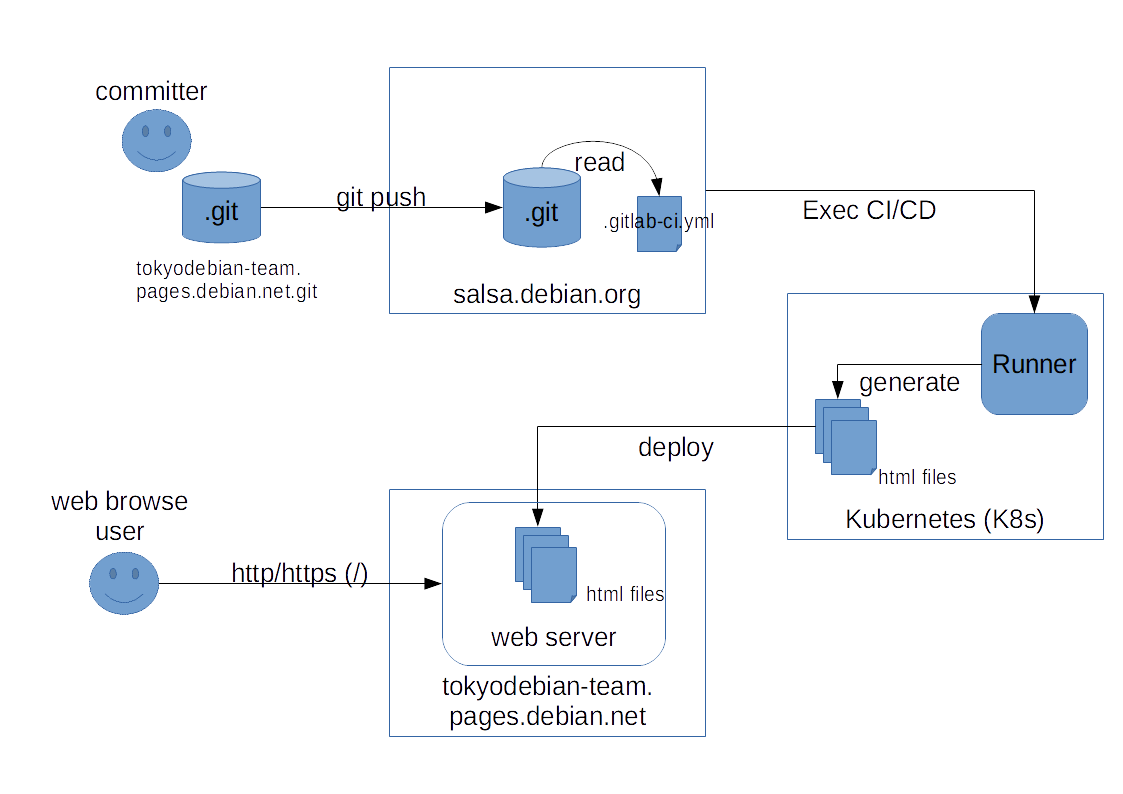
\includegraphics[width=12cm]{image201806/gitflow_web.png}
  \caption{webサイトへHTMLファイルを配備するCI/CD処理の流れ}
  \label{fig:deploy-html-CICD}
\end{center}
\end{figure}


\subsubsection{原稿システムの仕組み}

東京エリアDebian勉強会の原稿資料およびスライド資料のソースコードは、\url{https://salsa.debian.org/tokyodebian-team/monthly-report} のページにあります\footnote{関西Debian勉強会の資料もここにあります。}。


コンテンツはTeX(テフ)という組版システム\footnote{印刷を想定したレイアウトや文字、図などを配置して原稿を作成するシステムのことをいいます。}を利用しており、ソースコードであるtexファイルから中間ファイルのdviファイルを経て、最終的にpdfファイルを生成する仕組みになっています。配布している資料は、texのテンプレートを勉強会の有志が作成し、豊富な原稿の量は参加者の長年の積み重ねで支えられています。


salsaでは、texファイルを保存するgitリポジトリ"monthly-report.git"と、web公開するビルドしたpdfファイルを保存する"pdf20yy.git"というリポジトリに分けています\footnote{"pdf20xx.git"は、"pdf2005.git"から"pdf2018.git"まで存在しており、毎年増える予定です。}。これは、"monthly-report.git"でtexファイルをCI/CDの度にすべてビルドし直すには処理量が多すぎること、CI/CD処理が成功したとしてもpdfファイル数が多すぎてサーバ間のHTTP通信の送信可能サイズの上限を超えてエラーになることから\footnote{ERROR: Uploading artifacts to coordinator... too large archive id=11633 responseStatus=413 Request Entity Too Large status=413 Request Entity Too Large token=5ydbgD39}、一度のCI/CDで処理するpdfファイルの量を制限するためにリポジトリを年ごとに分割した経緯があります。


上記の転送ファイルサイズの制約を回避するため、salsaにおける原稿ファイルの生成からpdfファイルをweb公開するまでの処理は以下に流れになっています。


\begin{itemize}
  \item texファイルを保存している"monthly-report.git"をgit cloneしてtexファイルを作成する
  \item makeを実行し、pdfファイルが生成できることを確認する
  \item 原稿を完成させる
  \item texファイルをgit commitし、git pushする。push時にsalsaではCI/CD処理は実行しない
  \item make publishコマンドを実行し、pdfファイルを"pdf20yy.git"へgit commitし、git pushする
  \item "pdf20yy.git"でCI/CD処理を実行し、pdfファイルを"tokyodebian-team.pages.debian.net"に配備する
  \item webから"https://tokyodebian-team.pages.debian.net/pdf20yy/xxx.pdf"でファイルを取得できる
\end{itemize}


\begin{figure}[H]
\begin{center}
  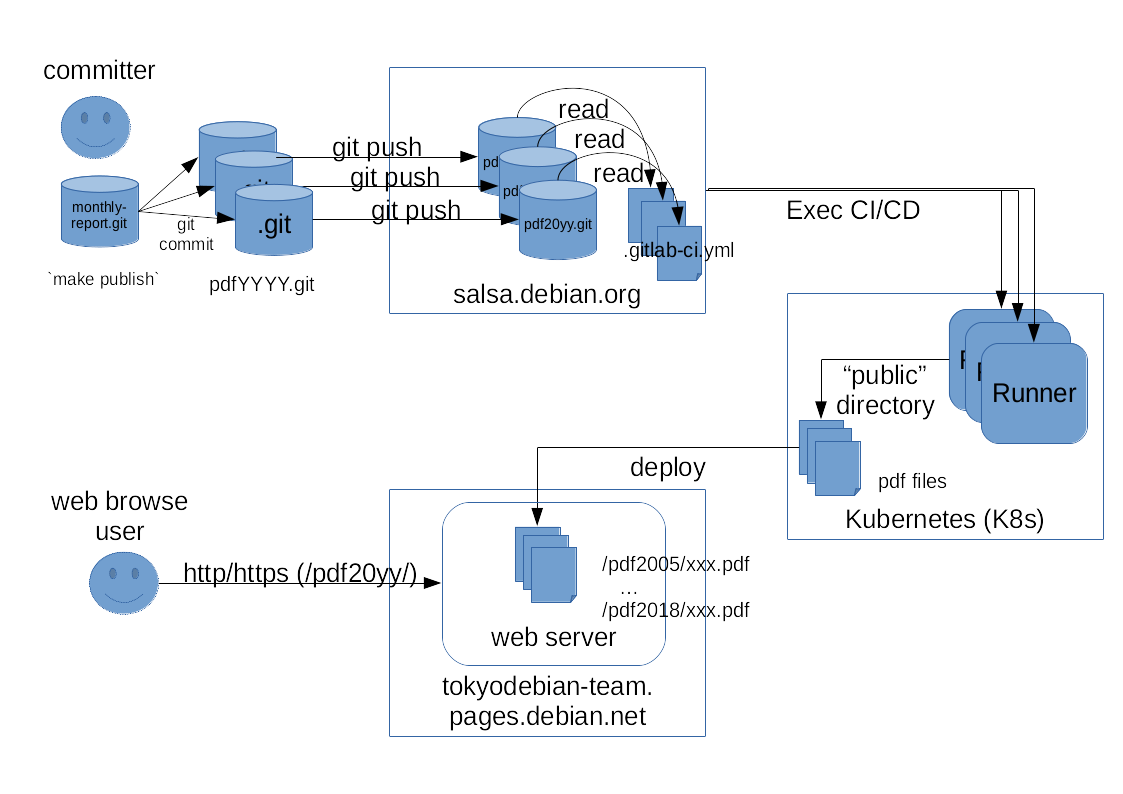
\includegraphics[width=12cm]{image201806/gitflow_pdf.png}
  \caption{webサイトへ原稿及びスライドPDFファイルを配備するCI/CD処理の流れ}
  \label{fig:deploy-pdf-CICD}
\end{center}
\end{figure}


\subsection{今後の課題}

原稿システムのCI/CD処理が失敗することもあり、Runnerや.gitlab-ci.ymlの設定を見直す必要があると考えています。

webサイトも原稿システムも作ってから年月が経過しているため、webサイトのリニューアルや原稿ファイルのUTF-8対応といった現代化をしていく重めの改修作業もあります。

また勉強会で発表していただいている方々も忙しいためか原稿を書いていただける方が減っており、半期のまとめ資料を冊子にしたときにページ数が少なくなってきている実情もあります。


\subsection{まとめ}

salsaで提供しているgitlabの機能と設定を紹介し、その機能を使って東京エリアDebian勉強会のシステムを移行した説明をしました。salsaを有効活用してDebianプロジェクトへ貢献することに繋がるとよいと思っています。

また、勉強会の参加者に原稿システムの理解を深めていただき、自分の学びになるだけでなく、他の参加者やインターネットで検索してきた方の学びにつながる勉強会にしていければよいと思っています。


%
% 冊子にするために、4の倍数にする必要がある。
% そのための調整
\dancersection{メモ}{}
\mbox{}\newpage

\vspace*{15cm}
\hrule
\vspace{2mm}

\includegraphics[width=2cm]{image200502/openlogo-nd.eps}
\noindent \Large \bf Debian 勉強会資料\\
\noindent \normalfont \debmtgyear{}年\debmtgmonth{}月\debmtgdate{}日 \hspace{5mm}  初版第1刷発行\\
\noindent \normalfont 東京エリア Debian 勉強会 (編集・印刷・発行)\\
\hrule

\end{document}
